%%%%%%%%%%%%%%%%%%%%%%%%%%%%%%%%%%%%%%%%%%%%%%%%%%%%
\section{Experiments}\label{sec:experiments}

All experiments were conducted on a single machine
(Apple M3 Pro, 18\,GB RAM) using Rust~1.82 release builds.
To measure \textit{pure computation time} independently of arrival
latency, we pre-load the full dataset and feed it $\Delta$ events
at a time, triggering each scan immediately after the previous completes.

%-----------------------------------------------------------------------
\subsection{EX-1: Scan Frequency Sensitivity}\label{sec:ex1}
%-----------------------------------------------------------------------

We quantify the effect of the scan frequency parameter $\Delta$ on total
processing time and characterize the tradeoff between output latency
and computational cost.
We varied $\Delta \in \{1, 10, 100, 1{,}000, 10{,}000\}$ on a synthetic
stream ($T = 10{,}000$, $|\mathcal{I}| = 20$, $W = 24$, $\theta = 10$;
see Appendix~A for generation details).

\begin{figure}[t]
\centering
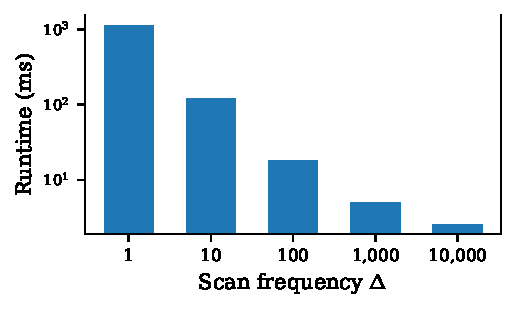
\includegraphics[width=\columnwidth]{ex1_h_vs_time.pdf}
\caption{Scan frequency $\Delta$ vs.\ processing time (log scale).}
\label{fig:ex1}
\end{figure}

As shown in Fig.~\ref{fig:ex1}, each 10$\times$ increase in $\Delta$ reduces
processing time by approximately one order of magnitude, confirming
that reducing scan count directly reduces processing cost.

%-----------------------------------------------------------------------
\subsection{EX-2: Scalability}\label{sec:ex2}
%-----------------------------------------------------------------------

We verify how processing time and peak memory usage scale as stream
length $T$ and item count $|\mathcal{I}|$ are varied independently.
We set $\Delta = T$ (batch mode) and measured pure computation time on
synthetic data ($\theta = 10$, $W = 120$), with baseline
$T = 10^5$ and $|\mathcal{I}| = 24$.

\begin{figure}[t]
\centering
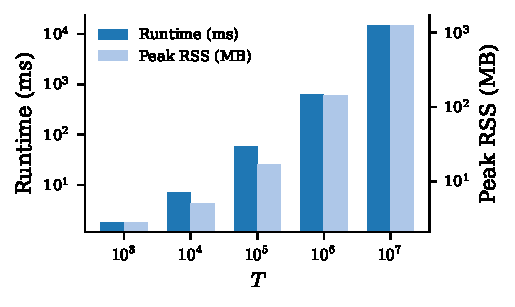
\includegraphics[width=\columnwidth]{ex2_scalability_T.pdf}
\caption{Scalability vs.\ $T$: Runtime and Peak RSS.}
\label{fig:ex2t}
\end{figure}

\begin{figure}[t]
\centering
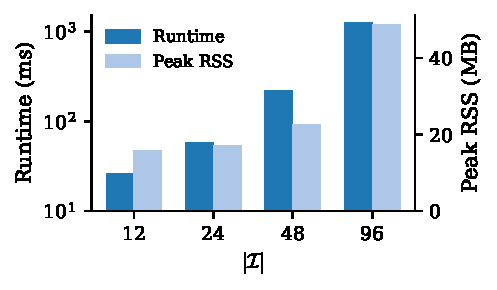
\includegraphics[width=\columnwidth]{ex2_scalability_N.pdf}
\caption{Scalability vs.\ $|\mathcal{I}|$: Runtime and Peak RSS.}
\label{fig:ex2n}
\end{figure}

As shown in Fig.~\ref{fig:ex2t}, runtime scales nearly linearly in $T$
(636\,ms at $T = 10^6$; 15{,}108\,ms at $T = 10^7$).
Fig.~\ref{fig:ex2n} shows super-linear scaling in $|\mathcal{I}|$
(1{,}272\,ms at $|\mathcal{I}| = 96$) due to the combinatorial growth
of higher-order candidates.
Peak RSS scales nearly linearly in $T$ and shows small dependence on
$|\mathcal{I}|$.

%-----------------------------------------------------------------------
\subsection{EX-3: Ablation Study}\label{sec:ex3}
%-----------------------------------------------------------------------

We quantify the independent contributions of Scan Stride Skipping and
Apriori Interval Pruning, and confirm the benefit of combining both.
We set $\Delta = T$ and measured pure computation time on synthetic data
($T = 100{,}000$, $|\mathcal{I}| = 48$, $W = 120$, $\theta = 50$,
epoch overlap 100) for four algorithm variants.

\begin{figure}[t]
\centering
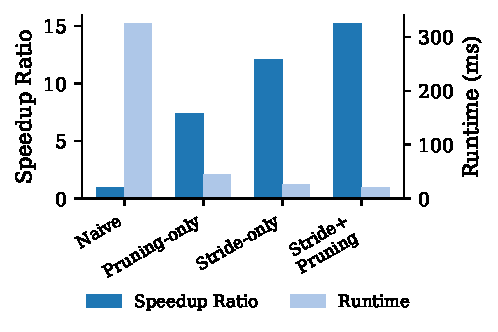
\includegraphics[width=\columnwidth]{ex3_speedup.pdf}
\caption{Ablation: speedup ratio relative to Naive.}
\label{fig:ex3}
\end{figure}

Fig.~\ref{fig:ex3} shows runtime and speedup ratios normalized to
Naive (1.00$\times$).
The Full variant (21.4\,ms) outperforms all individual configurations.
Scan Stride Skipping is the dominant contributor,
achieving a 12.1$\times$ speedup over Naive.
Apriori Interval Pruning alone achieves 7.4$\times$, and combining
both yields 15.2$\times$.
The two techniques contribute independently and complementarily.

%-----------------------------------------------------------------------
\subsection{EX-4: Application to CASAS Sensor Data}\label{sec:ex4}
%-----------------------------------------------------------------------

We apply the algorithm to real sensor streams to confirm that detected
dense intervals correspond to interpretable behavioral routines.
We use two series from the CASAS smart home
dataset~\cite{casas2013} (hh113 and mv001).
CASAS records motion and contact sensor activation streams from
residential environments, structurally analogous to autonomous agent
behavioral logs.
Sensor activations were aggregated into 15-minute time slots.
We set $W = 24$ slots ($= 6$\,hours) to capture activity routines
within specific blocks of the day (morning, evening, or night),
and $\Delta = W = 24$.
Table~\ref{tab:casas_stats} summarizes each dataset.

\begin{table}[t]
\caption{CASAS dataset statistics (slot width $= 15$\,min, $W = 24 = 6$\,h).}
\label{tab:casas_stats}
\begin{center}
\begin{tabular}{ccccc}
\hline
Dataset & $T$ & $|\mathcal{I}|$ & $\theta$ & Patterns \\\hline
hh113 & 48{,}901 & 7 & 14 & 26 \\
mv001 & 139{,}033 & 7 & 18 & 34 \\\hline
\end{tabular}
\end{center}
\end{table}

Representative patterns are listed in
Tables~\ref{tab:casas_hh113} and~\ref{tab:casas_mv001}.
For hh113, the most frequent pattern is the co-occurrence of
DiningRoom and Kitchen (meal preparation/dining), detected across
45 dense intervals.
The co-occurrence of Bathroom and Bedroom (wake/sleep routine)
was found in 8 intervals.
The three-item pattern DiningRoom + Kitchen + OutsideDoor (pre/post-outing
meal behavior) was detected in 7 intervals, showing that the algorithm
captures composite activity transitions.
For mv001, the co-occurrence of Bedroom and LivingRoom
(pre-sleep transition from living room to bedroom) was most frequent
with 113 intervals.
Kitchen and LivingRoom co-occurrence (post-cooking living room stay)
yielded 66 intervals, and the three-item pattern
Bedroom + Kitchen + LivingRoom (full evening-to-bedtime activity chain)
was detected in 44 intervals.

\begin{table}[t]
\caption{Representative detected patterns for hh113.}
\label{tab:casas_hh113}
\begin{center}
\footnotesize
\begin{tabular}{p{3.5cm}cp{2.0cm}}
\hline
Sensor combination & \#Int. & Inferred behavior \\\hline
DiningRoom + Kitchen               & 45 & Meal prep/dining \\
Bathroom + Bedroom                 &  8 & Wake/sleep routine \\
DiningRoom + Kitchen + OutsideDoor &  7 & Pre/post-outing meal \\\hline
\end{tabular}
\end{center}
\end{table}

\begin{table}[t]
\caption{Representative detected patterns for mv001.}
\label{tab:casas_mv001}
\begin{center}
\footnotesize
\begin{tabular}{p{3.5cm}cp{2.0cm}}
\hline
Sensor combination & \#Int. & Inferred behavior \\\hline
Bedroom + LivingRoom               & 113 & Pre-sleep: living$\to$bed \\
Kitchen + LivingRoom               &  66 & Post-cooking living stay \\
Bedroom + Kitchen                  &  44 & Wake/pre-sleep activity \\
Bedroom + Kitchen + LivingRoom     &  44 & Evening-to-bed chain \\\hline
\end{tabular}
\end{center}
\end{table}

The two datasets exhibit distinct behavioral characteristics.
In hh113, food-related patterns dominate, showing that daily routines
centered on the kitchen and dining room repeatedly form within 6-hour
windows.
In mv001, living room-to-bedroom transitions are most frequent,
suggesting that the pre-sleep sequence
(living room $\to$ cooking $\to$ sleep) is an established daily habit.
Bedroom + Office co-occurrence was also detected (23 intervals),
indicating a persistent remote-work pattern.
In both datasets, multi-item patterns ($k \geq 3$) were automatically
enumerated, revealing composite activity transitions not visible
from pairwise co-occurrence alone.
These results demonstrate that Streaming Apriori-Window automatically
detects meaningful behavioral routines from real sensor streams.
